\begin{frame}
	\frametitle{Introducci\'on}
	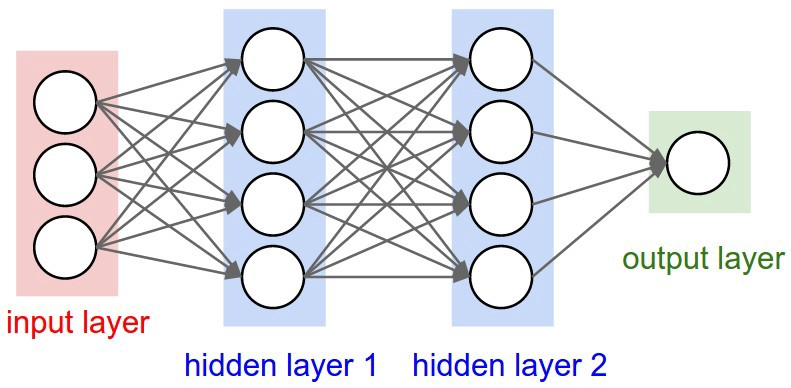
\includegraphics[scale=0.25]{topology}

	\begin{enumerate}
		\setbeamercolor{item projected}{bg=red!100!black,fg=white}
		\item Input Layers - La capa de entrada pasa los datos directamente a la primera capa oculta donde los datos se multiplican por los pesos de la primera capa oculta.
		\setbeamercolor{item projected}{bg=blue!100!black,fg=white}
		\item Hidden Layers - El trabajo de las capas ocultas es transformar las entradas en algo que la capa de salida puede usar.
		\setbeamercolor{item projected}{bg=green!100!black,fg=black}
		\item Output Layers - La capa de salida en una red neuronal artificial es la \'ultima capa de neuronas que produce resultados dados para el programa.
	\end{enumerate}

\end{frame}
